\documentclass[12pt]{article}
\usepackage[utf8]{inputenc}
\usepackage{cite}
\usepackage[spanish]{babel}
\selectlanguage{spanish}
\usepackage{graphicx}
\graphicspath{ {files/} }
\usepackage{url}
\usepackage{natbib}




\title{Reporte sobre la Actividad 4}
\author{García Parra Pedro}
\date{Febrero 2019}

\begin{document}

\maketitle

En esta actividad continuamos con el analisis de datos sobre el mismo archivo obtenido del Servicio Meteorológico Nacional.
Antes de comenzar con el análisis, primero resultó conveniente crear unas columnas extras las cuales digan el mes y año del dato para así poder hacer una serie de loops anidados los cuales faciliten o inclusp hagan posible realizar el análisis.
Una vez hecho ésto, las actividades fueron muy sencillas, gracias a la librería pandas se puedo hacer el análisis de los datos y con la libreria matplotlib se pudo hacer el análisis gráfico.

Para la primer actividad se utilizo un doble loop que recorria la lista 12 veces (una por cada mes) y guardaba los promedios de la lluvia acumulada durante todo el año. La gráfica de esta información aparece en la figura(\ref{fig:act1}). Podemos ver que los meses donde llueve más son de julio a septiembre, y durante los demás meses las precipitaciones se mantienen en el mismo nivel.

Para la segunda tambien se utilizó un doble loop con el cual se sumaban las precipitaciones anualmente. La grafica asociada a ésta actividad se puede ver en la figura(\ref{fig:act2}). Podemos ver que las precipitaciones se han mantenido mas o menos de la misma manera durante los 21 años de datos.

Para la tercer actividad se utilizaron dos triples loops los cuales recorren la lista acumulando los datos de la temperatura de cada año por mes obteniendo así una lista con una extencion de 12*(# de años de la lista). En la gráfica (figura \ref{fig:act3}) podemos ver que la temperatura ha fluctuado como una función senoidal, pero quizá no se vea un aumento de temperatura debido a la poca cantidad de datos.

Para la cuarta actividad se utilizaron los datos obtenidos en la actividad 3 pero ahora se visualizan en graficas de caja, como se muestra en la figura(\ref{fig:act4}). Para la quinta actividad se utilizó un loop que cada iteración genera un par de graficas de caja para así graficar todos los años.

\begin{figure}
    \centering
    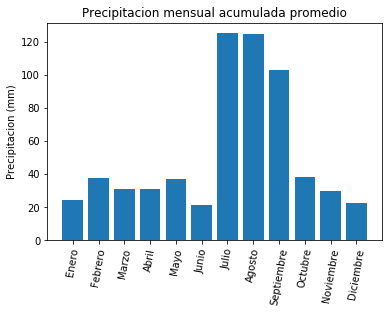
\includegraphics[scale=.8]{act1.png}
    \caption{Precipitación mensual acumulada promedio de la colección de datos de Obregón}
    \label{fig:act1}
\end{figure}
\begin{figure}
    \centering
    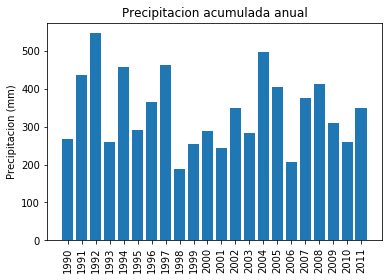
\includegraphics[scale=.8]{act2.png}
    \caption{Precipitación acumulada para cada año de Cd. Obregón}
    \label{fig:act2}
\end{figure}
\begin{figure}
    \centering
    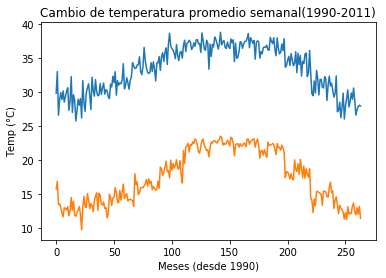
\includegraphics[scale=.8]{act3.png}
    \caption{Temperatura máxima y mínima en la misma figura, como función del tiempo de Cd. Obregón}
    \label{fig:act3}
\end{figure}
\begin{figure}
    \centering
    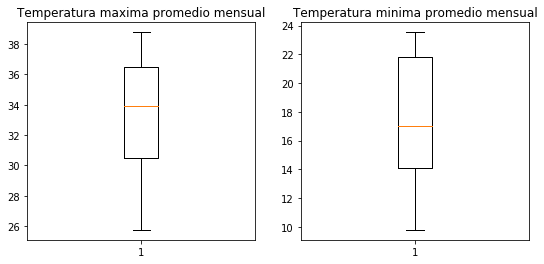
\includegraphics[scale=.8]{act4.png}
    \caption{Temperatura promedio mensual para la temperatura mínima y máxima por separado}
    \label{fig:act4}
\end{figure}
\end{document}
